% -*- program: xelatex -*-
\documentclass[12pt]{report}
\pagenumbering{arabic}

\widowpenalty=9999
\usepackage[normalem]{ulem}
\usepackage{setspace}
\usepackage[english]{babel}
\usepackage[letterpaper, margin=1in]{geometry}

\usepackage{fontspec}
\setmainfont{Heuristica}

\usepackage{booktabs}
\usepackage{graphicx}
\usepackage[table,x11names]{xcolor}
\usepackage{hyperref}
\usepackage{float}

\begin{document}

\title{Exploring the Use of Machine Learning-based Genome Wide Association Studies 
of Adolescent Idiopathic Scoliosis}

\author{Allie Burton\\Advisor: Prof.\ Sandra Batista}

\date{}
\maketitle

\doublespacing

\tableofcontents

\abstract{Scoliosis is a disease marked by curvature of the spine. The most common type,
adolescent idiopathic scoliosis (AIS), generally occurs right before puberty and
has no known causes. According to the Scoliosis Research Society, approximately
30\% of all AIS patients have some family history of scoliosis, so many researchers
now are looking for a genetic component\cite{ScoliosisResearchSociety}. To look
for these genetic components, researchers perform what is known as a genome-wide
association study, or GWAS, which the National Human Genome Research Institute
defines as an ``approach that involves rapidly scanning markers across the
complete sets of DNA, or genomes, of many people to find genetic variations
associated with a particular disease''\cite{NationalHumanGenomeResearchInstitute2015}.
The results of these studies, however, have been generally inconclusive collectively.
The goal of my project is to study the usage and efficacy of machine learning 
for GWAS in scoliosis in an effort to affirm previous results or discover new ones.}


\chapter{Introduction}
Approximately 4\% of all children between the ages of 10 and 18 are diagnosed with
adolescent idiopathic scoliosis\cite{ScoliosisResearchSociety}. I was one of them. 
At the age of 10, I was diagnosed after my mother noticed that my shoulders were 
uneven. Like many other children diagnosed with scoliosis, I wore a back brace 
for several years until I stopped growing. Unfortunately, my curve continued to
progress throughout puberty, and although it has stopped progressing now, I still
have a curve of approximately 40 degrees.

Naturally this sparked a personal interest in the causes of adolescent idiopathic
scoliosis, which is why I chose to study the possibility of discovering potential 
genetic sources of AIS via machine learning-based genome-wide association studies.
Although I was unable to test my theories on scoliosis data due to time constraints
and study participant privacy protections, I believe that the information presented
here is applicable to future genome-wide association studies of AIS.

\begin{figure}[H]
    \caption{My x-ray from 2008, age 13}
\label{Figure 1}
    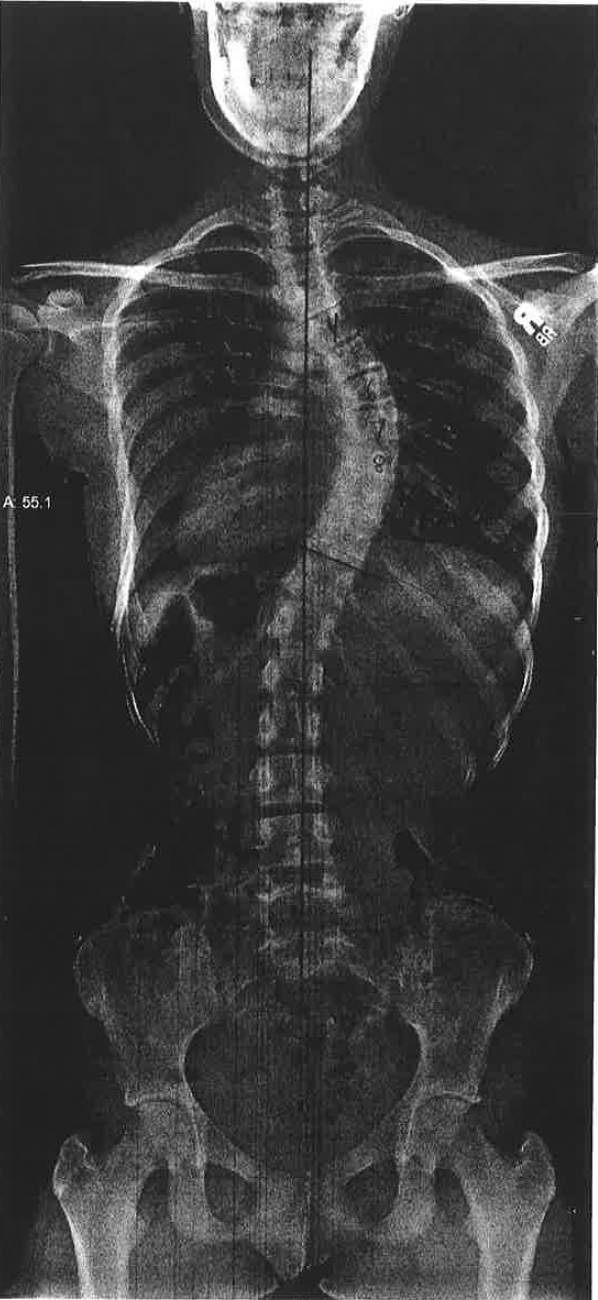
\includegraphics[height=8in]{xray.png}
    \centering
\end{figure}


\chapter{Background}

\section{Important Terminology}
To conduct a genome-wide association study (GWAS), researchers get DNA samples from two
groups of people: those with the trait in question and those without it. Using
these samples, each person's entire genome is scanned in a machine looking for
single-nucleotide polymorphisms. A single-nucleotide polymorphism, or SNP
(pronounced ``snip''), is a variation at a single position in an individual's
DNA sequence that occurs in one percent or less of the population. If certain
SNPs occur more frequently in persons with the disease than without it, then
those SNPs are associated with the trait. Although these SNPs can point to places
in the human genome that might be related to the source of the trait, the SNPs
themselves may not be the cause of the trait itself, so researchers often look
at base pairs in the region to see if they are also related\cite{NatureEducat}.
The most common method of statistical analysis for GWAS is logistic regression
where the dependent variable is case-control status and the independent variable
is a specific SNP genotype. ``The output of a logistic regression is identity of
the reference allele and an odds ratio with its standard error (or confidence
intervals) along with a statistic and p-value that test whether the odds ratio
differs from unity''\cite{Corvin2010}. A logistic regression is performed for
each SNP, often totaling to well over 500,000 logistics regression per study.

\section{Related Work}
\subsection{Machine Learning-Based Genome-Wide Association Studies}
Although there have not been any studies done to date using machine learning for
GWAS of idiopathic scoliosis, there have been many studies using machine learning
for other phenotypes including IgM and rheumatoid arthritis, as mentioned above,
in addition to myocardial infarction, coronary artery calcification, and anti-cyclic
citrullinated peptide\cite{Szymczak2016}. These studies will provide the inspiration
for my methodology, specifically D’Angelo et.\ al.’s\cite{DAngelo2009} and Tang
et.\ al.’s\cite{Tang2009} GWASs of rheumatoid arthritis and Stassen et.\ al.’s
GWASs of IgM.

\subsection{Scoliosis Genome-Wide Association Studies}
% TODO: include at least one paragraph for each study referenced

Sharma et.\ al.\ conducted the first genome-wide association study of AIS in 2011 
on approximately 400 United States families and subsequently conducted three
replication studies with varying numbers of participants and ethnic backgrounds.
They found 100 SNP associations that set the baseline for later studies.

Later in 2011, Takahashi et.\ al.\ conducted another GWAS of AIS, this time with
approximately 1,400 Japanese females using 87 of Sharma et.\ al.'s top 100 SNPs.
However, this study only found 1 of the 87 to be significant. The most significant
SNP they found was located on chromosome 10 near a locus not seen in other studies.
This locus, LBX1, was significant because genes in similar places in other animals,
specifically mice and fruit flies, were connected to the dorsal spine.

Later studies did not show much congruence with these or each other, although 
SNPs close to or related to LBX1 show the most promise\cite{Zhao2015}.


\section{Suitability of Machine Learning for Genome-Wide Association Studies}
The data that comes from a standard GWAS is well suited for a machine learning task.
GWAS best fits under the subcategory of supervised learning, which requires samples,
features, and targets in its training set. In this case, each study participant 
would be a sample, the SNPs would be features, and the targets would be the participants'
respective affection status.


% TODO: cite Mieth paper 
% TODO: cite Botta paper
% TODO: cite Szymczak
% TODO: maybe talk about classification vs. regression models and usefulness

\section{Machine Learning Methods}
\subsection{LASSO}
\subsection{Random Forest}

% TODO: Standard of evidence

\chapter{Methods}
\section{Phase 1}
The purpose of Phase 1 was to familiarize myself with using PLINK, an open-source
command-line ``whole genome association analysis toolset''\cite{Chang}. For this
phase, I used the GAW16 data set from the North American Rheumatoid Arthritis
Consortium. This data set contains 868 cases of rheumatoid arthritis and 1,164 
controls for a total sample size of 2,062. This data set came in two parts: 
a CSV file and a MAP file. The CSV file contains 2,062 records each with the 
following fields:
\begin{itemize}
    \item{subject ID}
    \item{Rheumatoid arthritis (RA) affection status}
    \item{gender}
    \item{HLA-DRB1 allele 1}
    \item{HLA-DRB1 allele 2}
    \item{number of shared-epitope alleles}
    \item{existence of shared-epitope alleles}
    \item{anti-CCP}
    \item{rheumatoid factor IgM}
    \item{545,080 SNP-genotype fields}
\end{itemize}
Of these fields the most relevant for my purposes are the RA affection status,
and the SNP-genotype fields. The .map file is a special type of file used by
PLINK that contains information on each of the 545,080 SNPs with these fields:
\begin{itemize}
    \item{SNP name}
    \item{chromosome}
    \item{SNP position in base pairs}
\end{itemize}

In order to ensure compatibility with PLINK, the CSV file needed to be
reformatted to .ped format, the standard file format for PLINK.\@ This
pre-processing consisted of removing the fields corresponding to HLA-DRB1
alleles, number of shared-epitope alleles, existence of shared-epitope alleles,
anti-CCP, and rheumatoid factor IgM;\@ rearranging columns 1-3; changing the
denotation for male and female from ``M'' and ``F'' to ``1'' and ``2''; and
reformatting the denotation for genotypes. I used Python and the command-line
utility sed to reformat the data.

After pre-processing the data, I used PLINK to run a GWAS using logistic
regression (the traditional method) and LASSO.\@ I used R\cite{RCoreTeam2016} to
call PLINK and generate the visualizations of the results.

\section{Phase 2: Scoliosis Data Analysis}
We requested the genotype data from the Takahashi study in Japan in October and
finally received it in April. Unfortunately the data was in summary format listing
by SNP how many people had a specific genotype and whether they were case or control.
Despite this setback, I still wanted to do some sort of analysis with the data I
had received, even though it would not be based in machine learning.

The data contained information on 605,479 SNPs, including number of case and 
control participants and statistical information. For my analysis, I used all SNPs
and the case and control columns corresponding to each allele and the chromosome
number.

% TODO: Find some fancy way to represent this as an equation
Following the general theme of a genome-wide association study, for each SNP I 
compared the proportion of case participants of each genotype with the proportion
of control participants of each genotype, looking for significant differences in 
percentages, which I defined as being at least two standard deviations away from
the mean difference in percentages.

To conduct this analysis, I used Python 3.6 with the packages pandas\cite{pandas}
and NumPy\cite{numpy} for data processing and joblib to parallelize the script. I ran
the script on Princeton's supercomputer Della.


\chapter{Results}
\section{Phase 1: Rheumatoid Arthritis Data Analysis}
With the logistic regression, there was no consistency with the Tang study
results for a number of reasons, primarily using different classification
methods (logistic regression vs.\ random forests). There was, however, a little
consistency between the logistic regression results and the LASSO results. The
LASSO results also shared one SNP that was in the top 10 SNPs in the Tang study.
The SNP in common between my PLINK log regression and LASSO runs is highlighted
in light blue, and the SNP in common between the Tang study and my LASSO run is
highlighted in green. Interestingly, all of the top 138 SNPs in my log regression
were from chromosome 6, which has been linked to rheumatoid arthritis previously
\cite{RAgene_manchester}\cite{RA_haplotypes}.


\begin{table}[!ht]
\centering
\caption{PLINK Log Regression vs. Tang Random Forest}
\label{Table 1}
\begin{tabular}{@{}ll@{}}
\toprule
PLINK Log Regression & Tang Random Forest \\ \midrule
\cellcolor{PaleTurquoise2}rs2395175            & rs2074488          \\
rs660895             & rs9461680          \\
rs6910071            & \cellcolor{PaleGreen2}rs2476601          \\
rs2395163            & rs2523619          \\
rs3763309            & rs3093662          \\
rs3763312            & rs3761847          \\
rs9275224            & rs2156875          \\
rs2395185            & rs2395471          \\
rs2516049            & rs13207315         \\
rs477515             & rs7026551          \\ \bottomrule
\end{tabular}
\end{table}

\begin{table}[ht]
\centering
\caption{PLINK LASSO Results}
\label{Table 2}
\begin{tabular}{@{}lll@{}}
\toprule
SNP        & Allele 1 & Effect   \\ \midrule
\cellcolor{PaleTurquoise2}rs2395175  & A        & 0.186673 \\
rs660895   & G        & 0.091164 \\
rs9275595  & G        & 0.064551 \\
rs9275555  & A        & 0.032611 \\
rs2900180  & A        & 0.026195 \\
rs10484560 & A        & 0.222120 \\
\cellcolor{PaleGreen2}rs2476601  & A        & 0.021363 \\
rs6910071  & G        & 0.021057 \\
rs10953244 & C        & 0.009081 \\
rs606537   & A        & 0.005849 \\ \bottomrule
\end{tabular}
\end{table}

The results from the logistic regression are also shown in this Manhattan plot.
The highest SNP in the plot, rs2395175, is the most statistically significant.

\begin{figure}[H]
    \caption{Log Regression Results}
\label{Figure 2}
    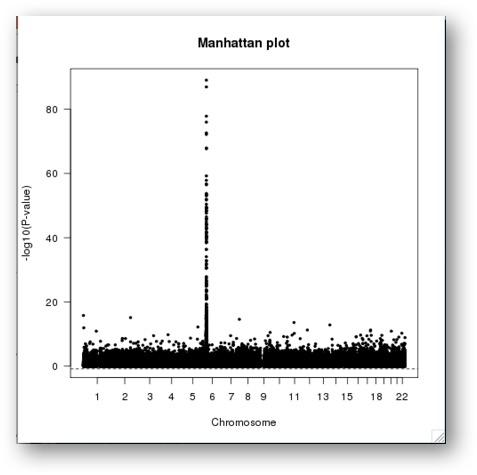
\includegraphics[width=8cm]{figure_1}
    \centering
\end{figure}


% TODO: insert results here
% TODO: ERROR ANALYSIS


\chapter{Discussion and Conclusion}



\bibliographystyle{ieeetr}
\bibliography{Thesis}

\end{document}
